\section{Forums}
\subsection{Overview}
Forums are a common feature in learning management systems as it provides a community environment where students can ask questions and discuss content with educators and other students.
Many of these built-in forums, however, are very basic and lack sufficient search, sorting and filtering functionality.
In many cases, educators are turning to external, third-party forums in order to take advantage of the more advanced features that they offer.

The aim of this feature is to develop a built-in forum that meets students' and educators' needs so that they no longer need to use an external application.

The forum interface consists of the overview page and the individual post pages.

\subsubsection{Forum Overview Page}

In general, the forum overview page consists of a list of posts, as well as search and filtering mechanisms.
The collapsible filter menu allows users to filter the forum posts based on pre-defined tags.
Forum posts are ordered such that the list of pinned posts are at the top, followed by the remaining posts in chronological order.
Each row in the table includes the post title, date created, number of replies, number of comments and the associated tags.

\begin{figure}[h!]
    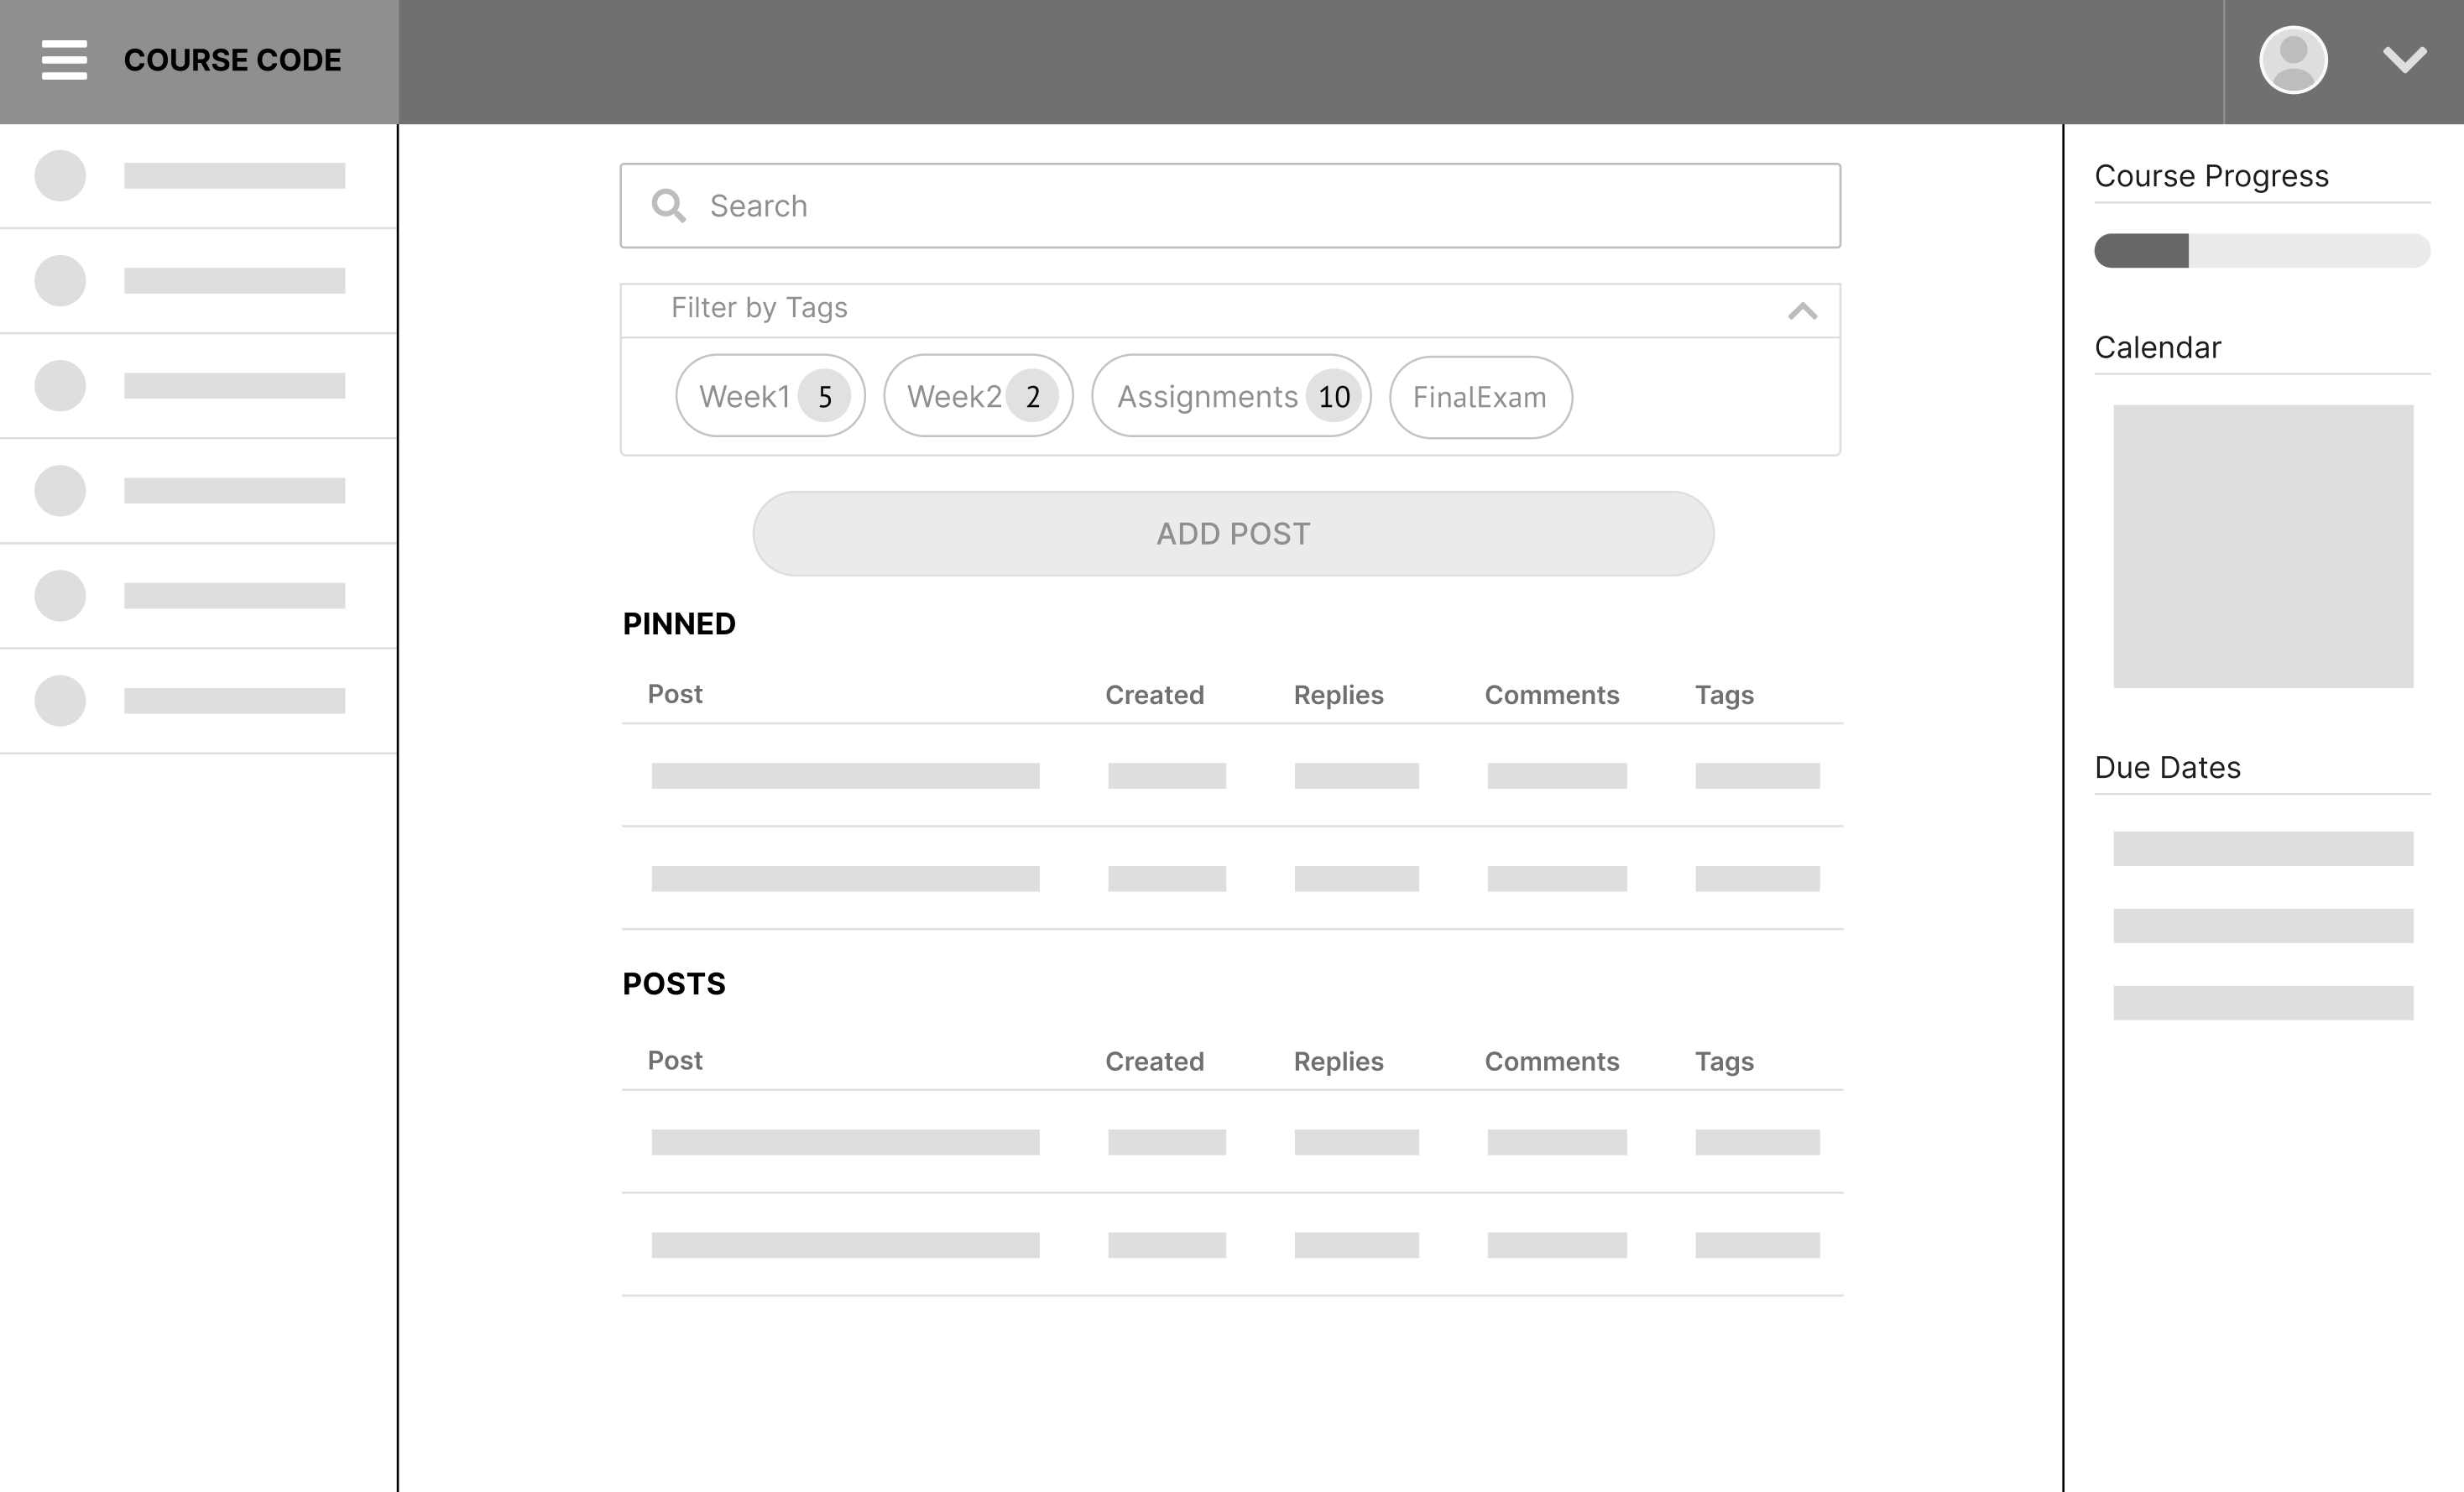
\includegraphics[scale=0.2]{forum-overview-page-student.png}
    \centering
    \caption{Forum overview page for a student.}
\end{figure}

\newpage

Staff have an additional button that allows them to pin and unpin posts.

\begin{figure}[h!]
    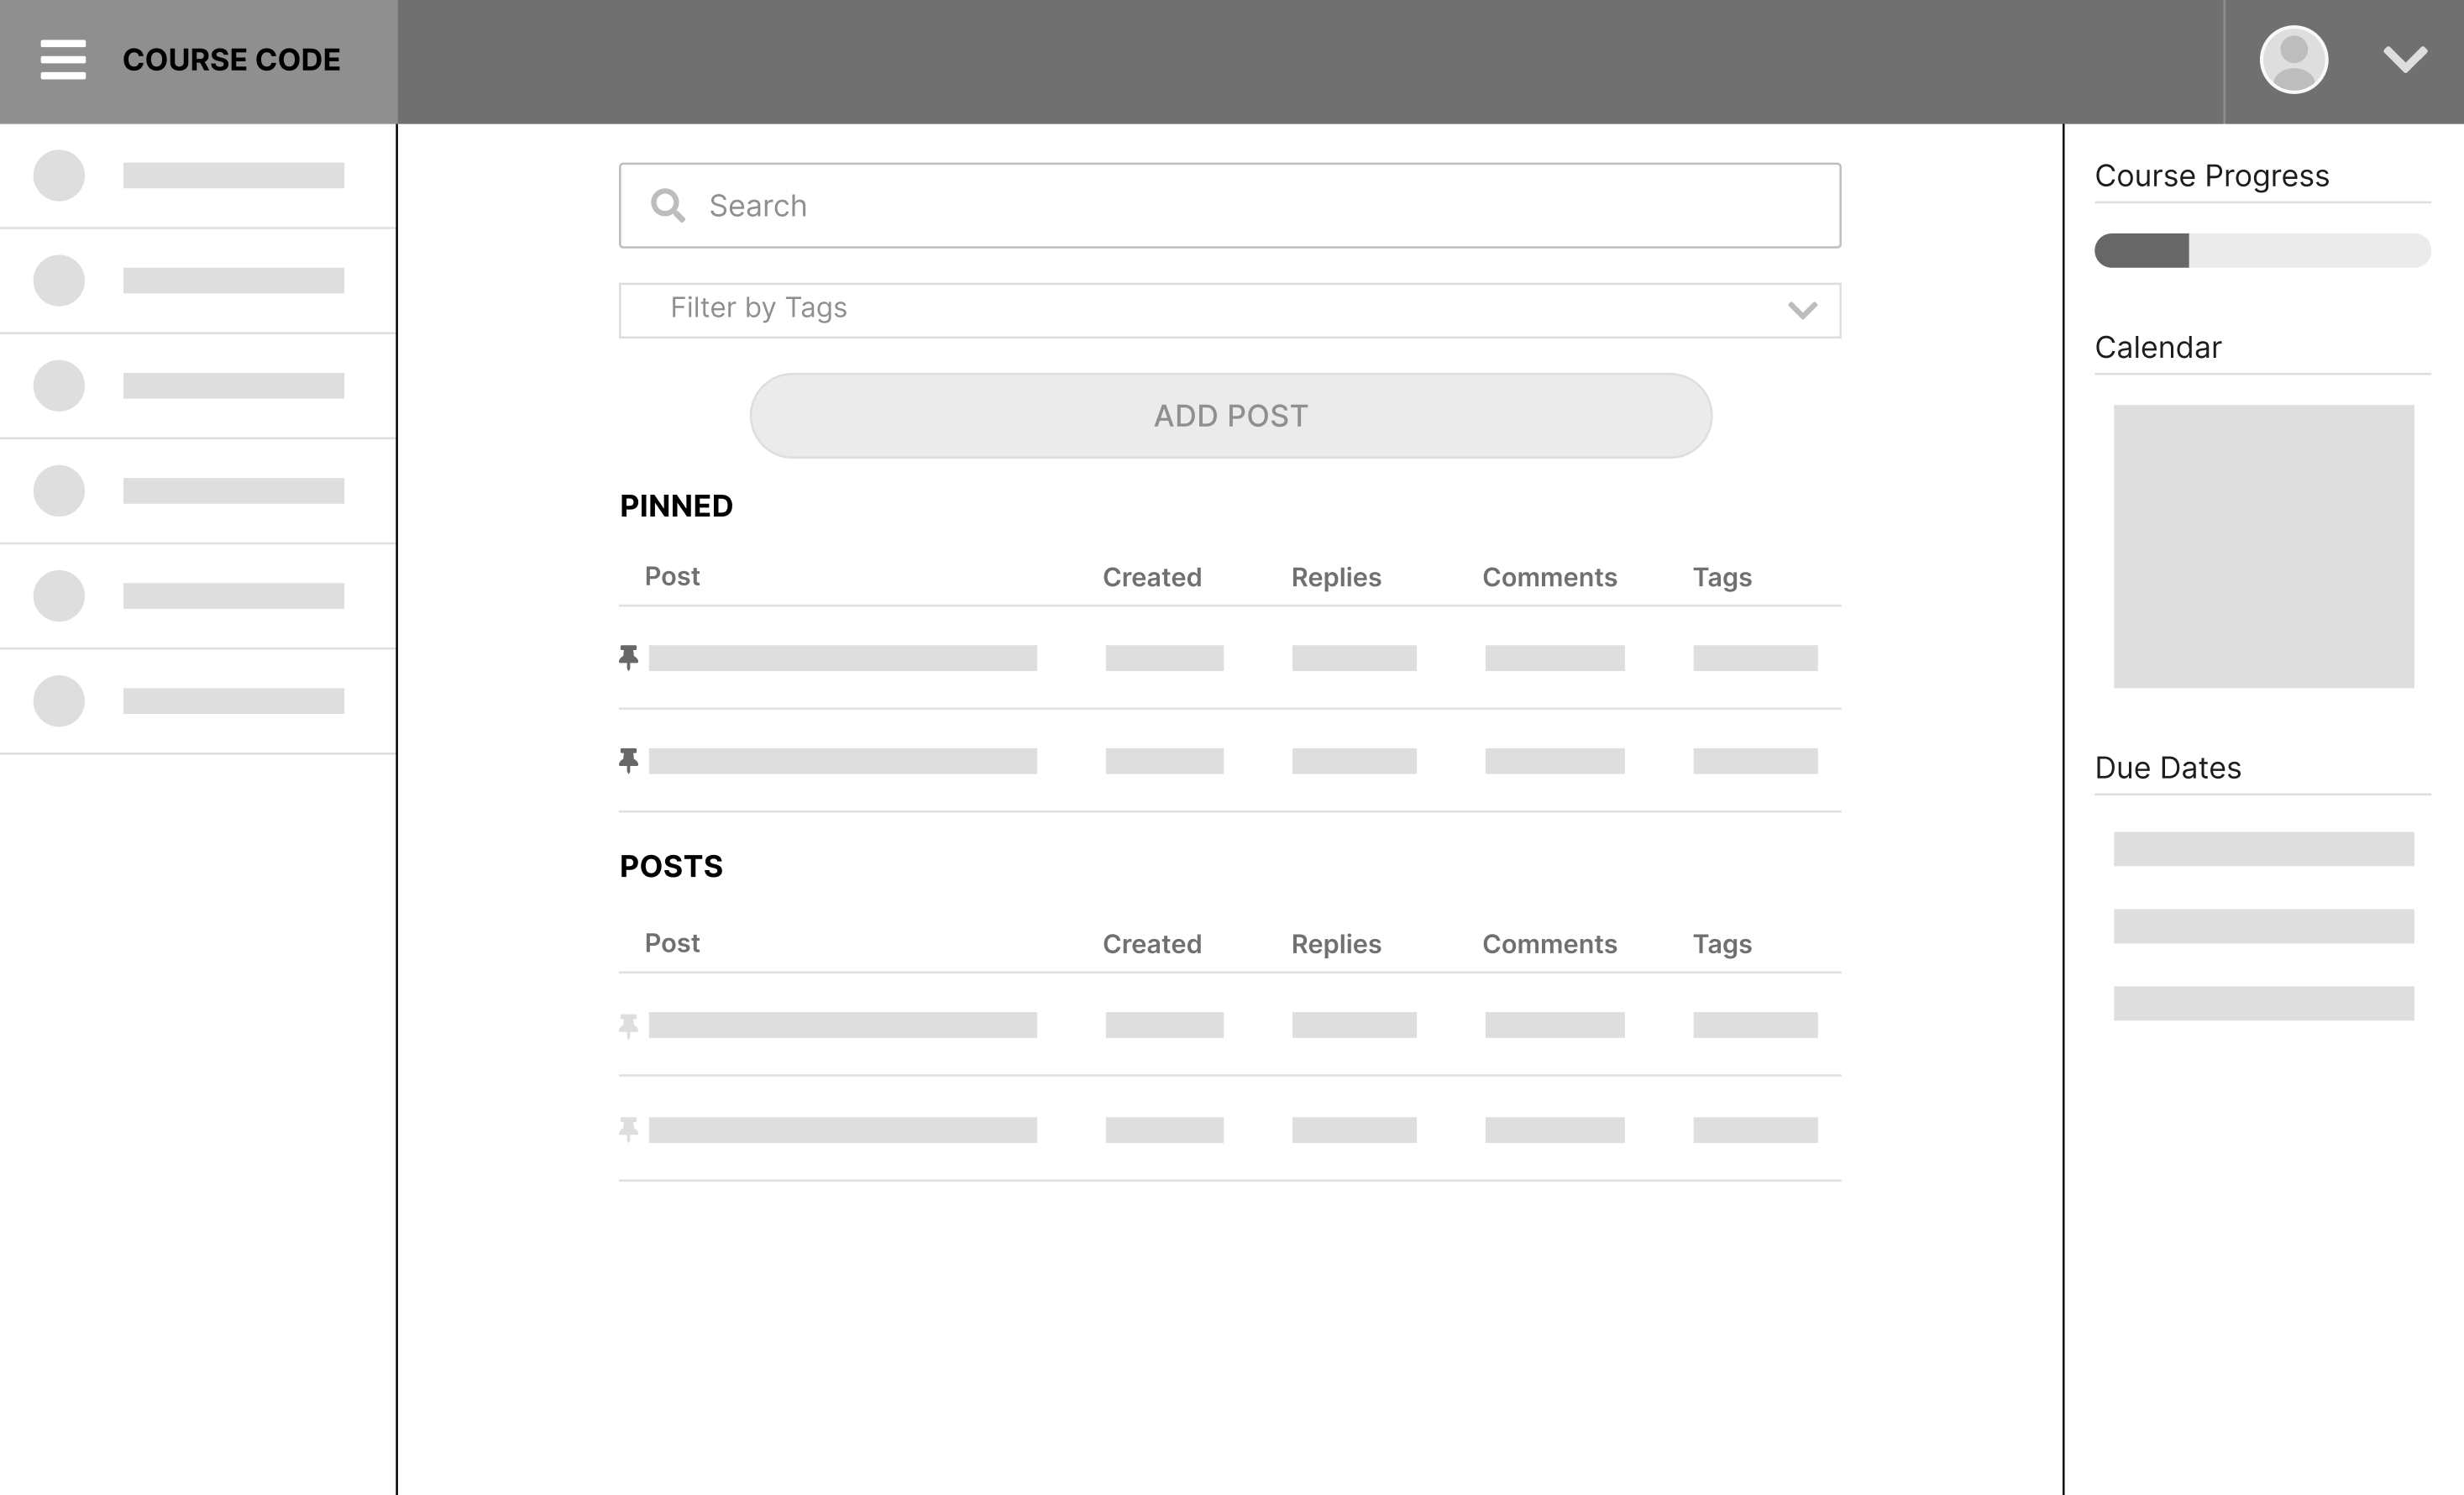
\includegraphics[scale=0.2]{forum-overview-page-admin.png}
    \centering
    \caption{Forum overview page for an admin.}
\end{figure}

\subsubsection{Post Page}

\begin{figure}[h!]
    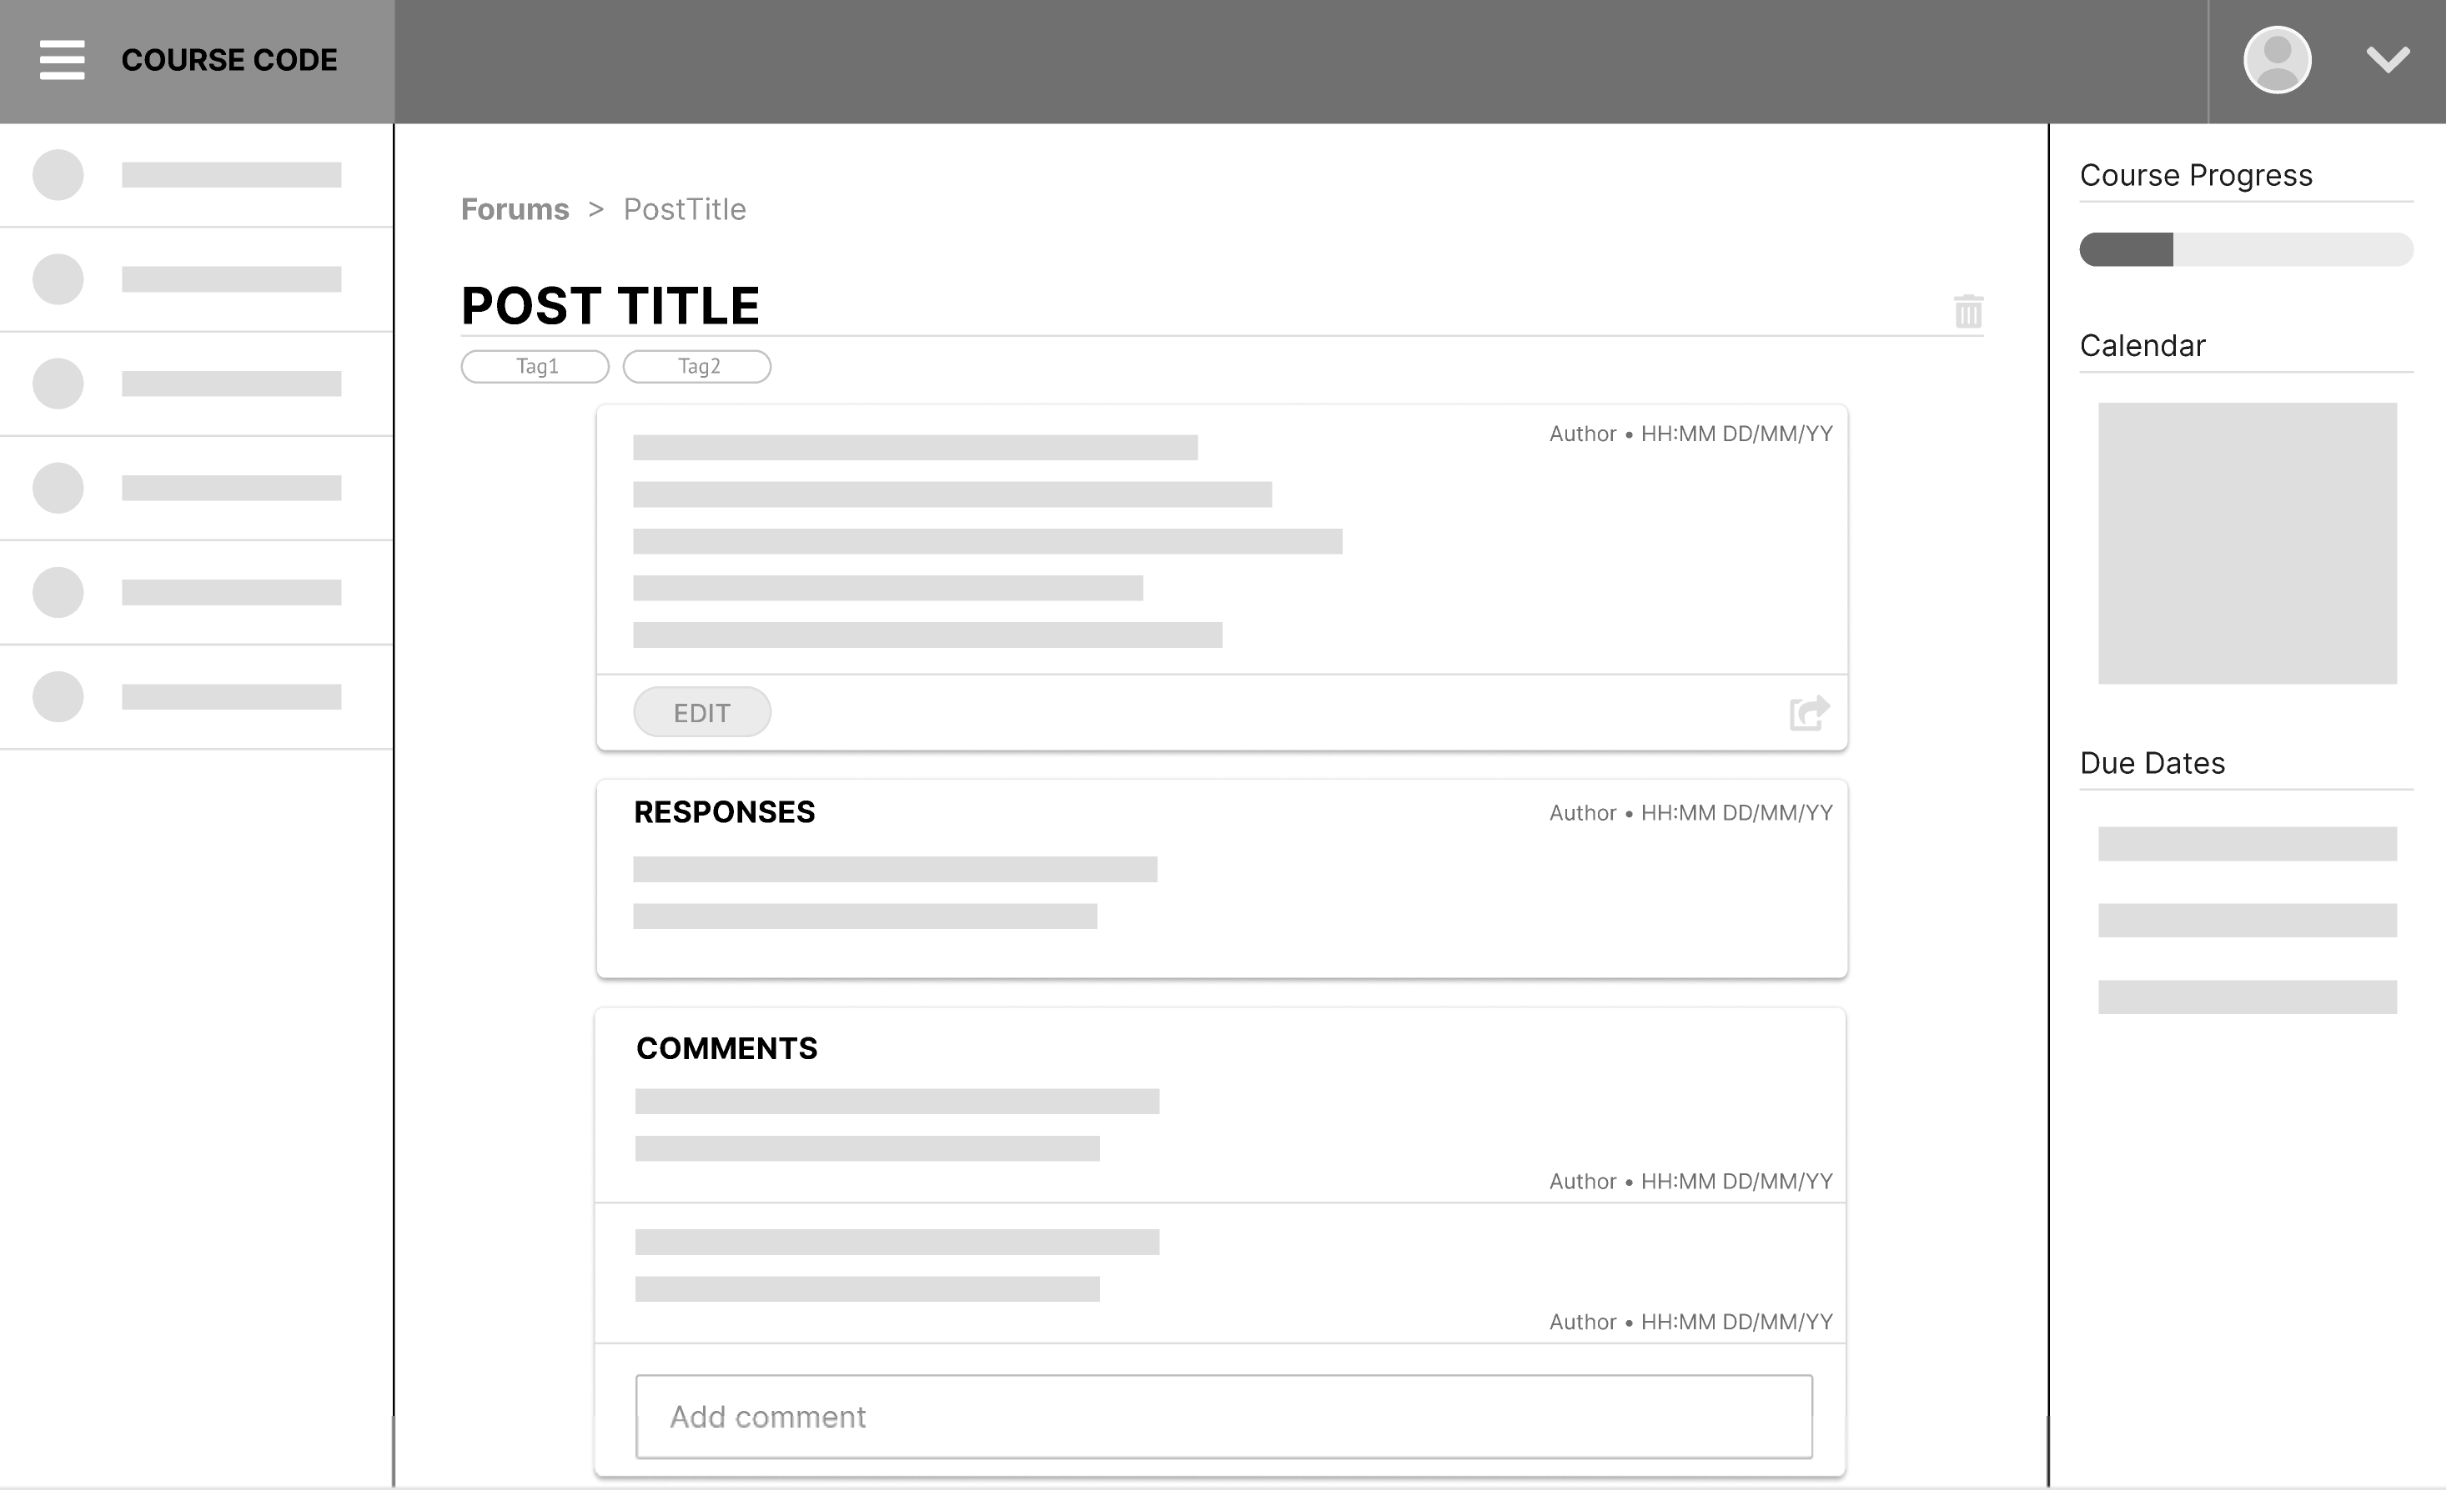
\includegraphics[scale=0.2]{forum-post-page-answered-student.png}
    \centering
    \caption{Forum post page for a student.}
\end{figure}

Each forum post has its own post page which contains the post details, responses and comments.
Students are able to edit their posts from the post page if required.
They can easily view the instructor's response, if any, in the responses section.
The comments section allows the author to view and leave any additional comments.
It also gives other students a place to write a response or ask questions based on that forum post.

\newpage

\begin{figure}[h!]
    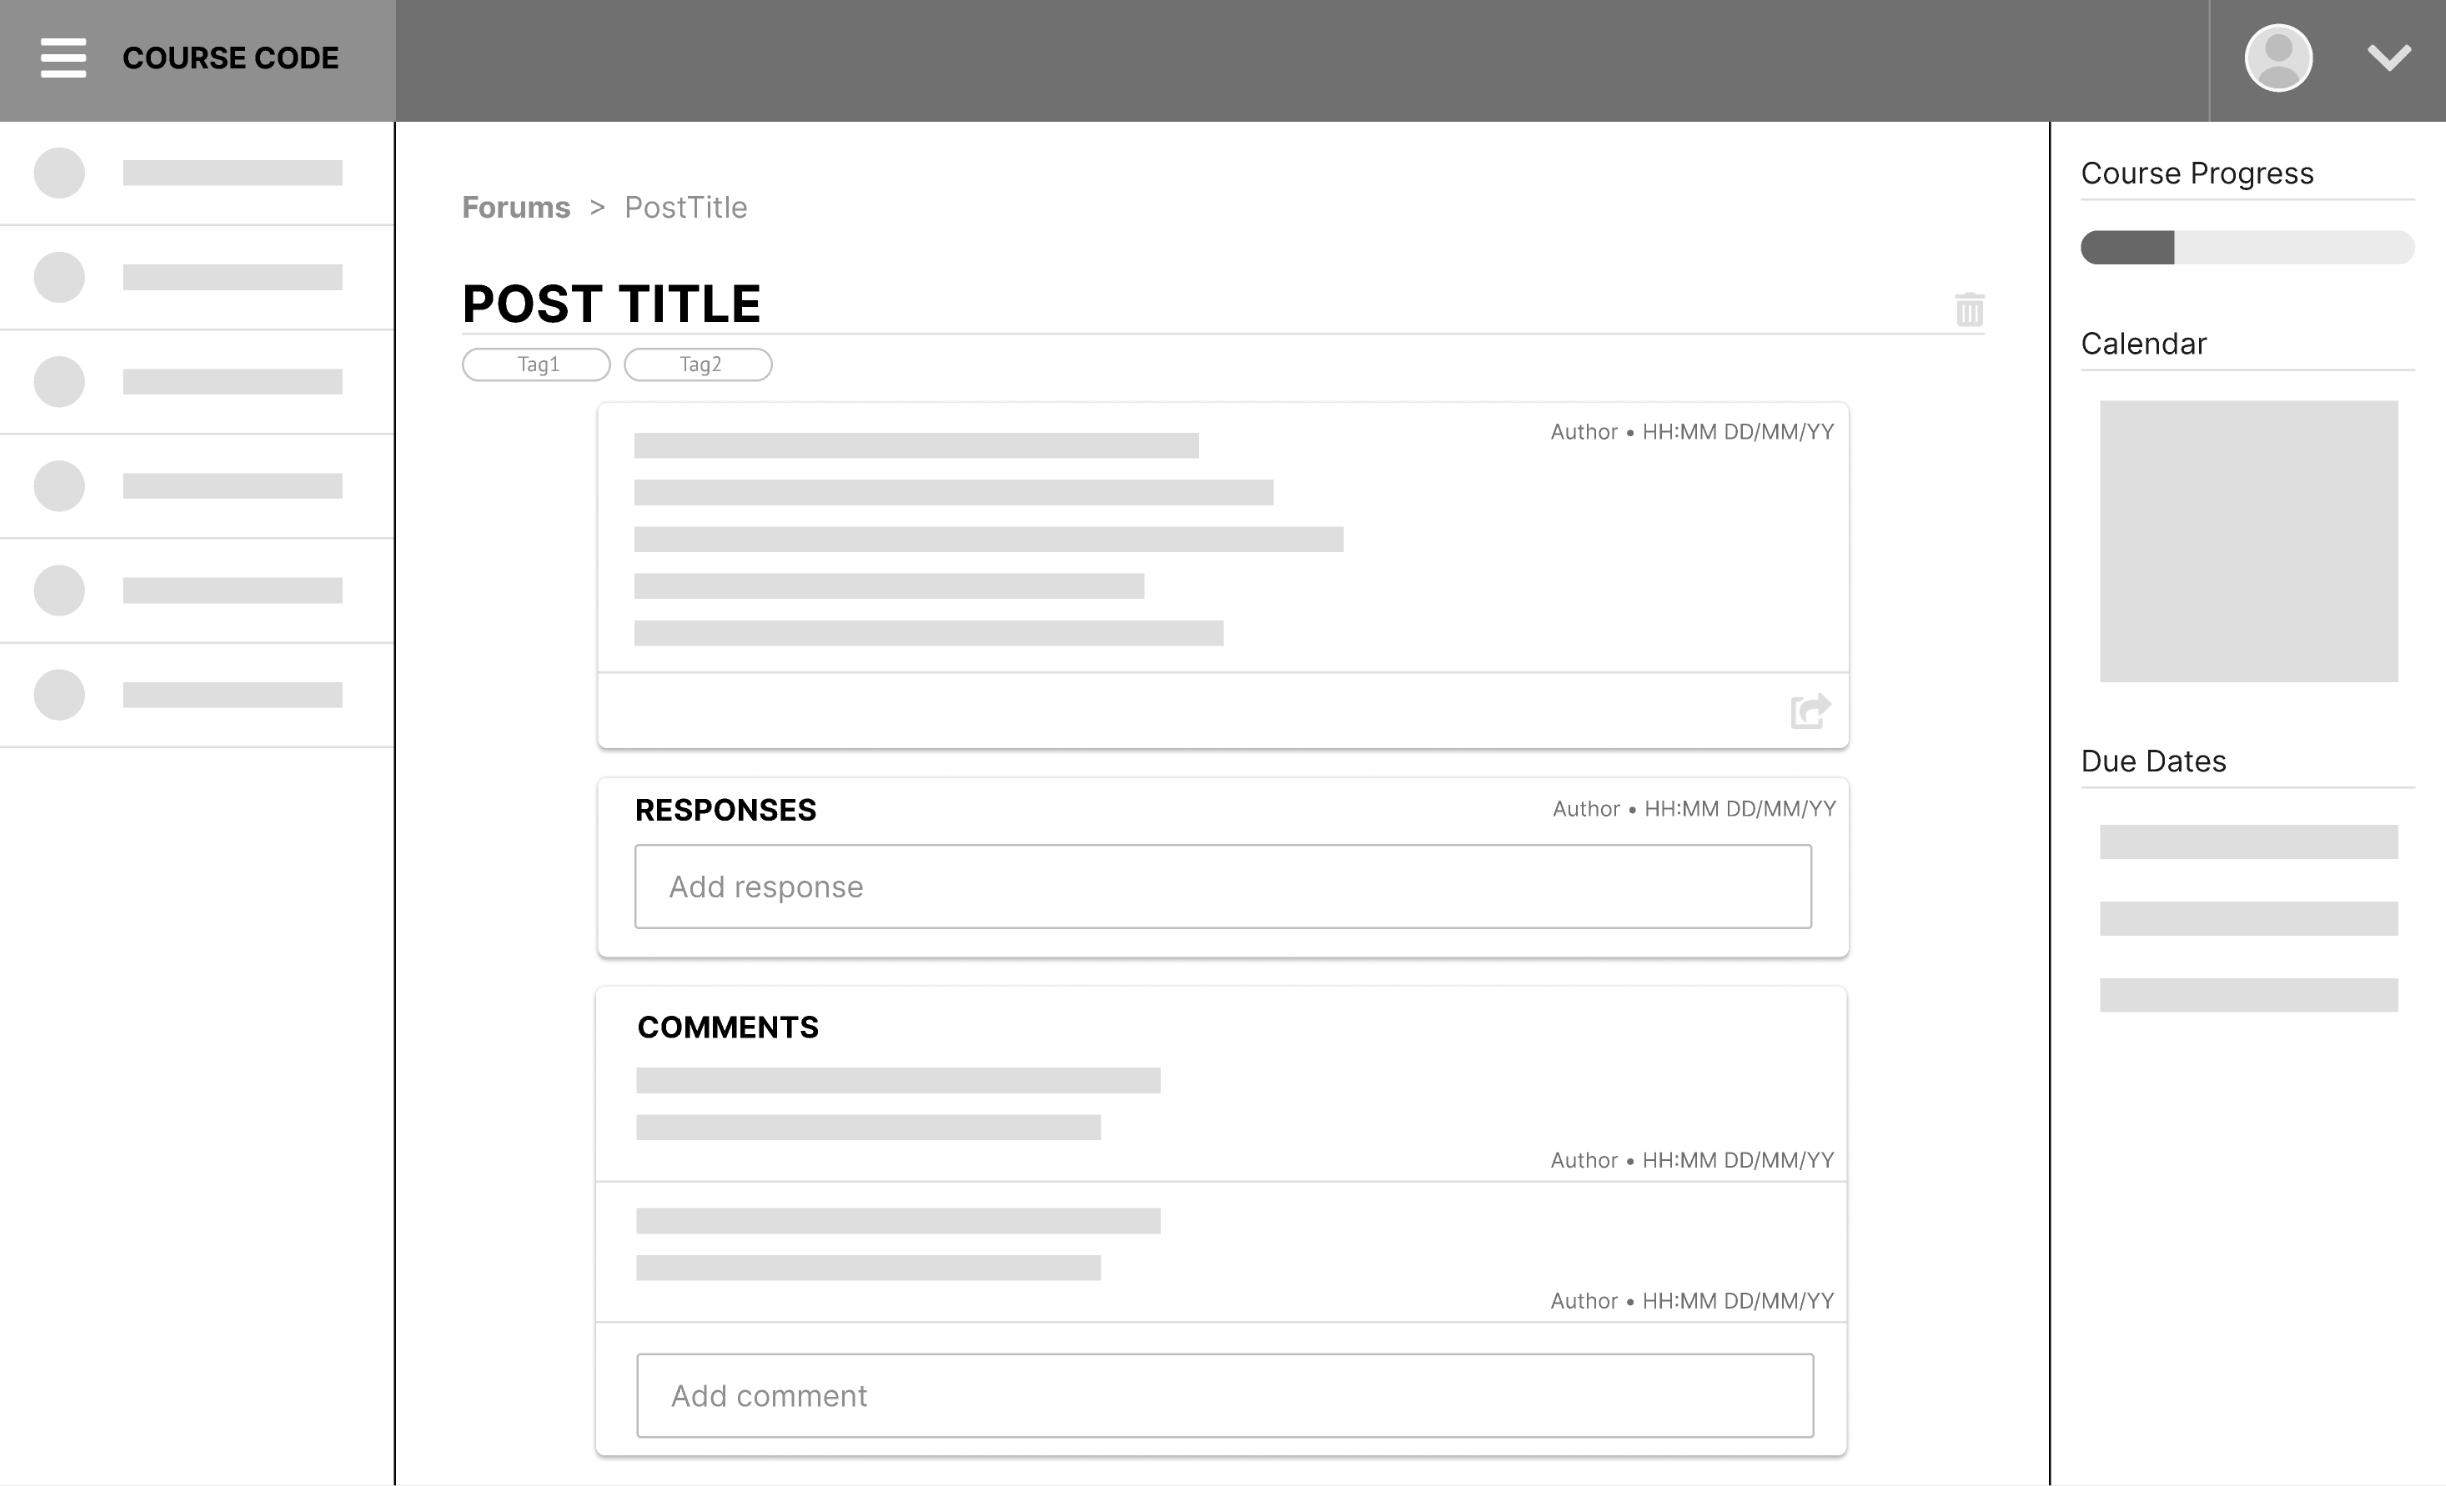
\includegraphics[scale=0.2]{forum-post-page-unanswered-admin.png}
    \centering
    \caption{Forum post page for an admin.}
\end{figure}

If a forum post is unanswered, an admin is able to leave a response.
The current idea is to restrict this so that only Staff can write responses to ensure that all responses are verified.
It also ensures that forum posts aren't left unanswered if a student accidentally leaves a follow-up question in the responses area, instead of the comments section.
This method of implementation may be reassessed if time allows.

\subsection{Additional Features}
As a result of reaching major milestones quicker than expected when building the forum component, additional features were able to be implemented to enhance the functionality and usefulness of the forums.

\subsubsection{Sortable Table}
To provide more methods to help users with finding specific posts, sorting functionality was added to the post tables on the forum overview page.
Users can click on the headings of each column in the table to toggle the sort order based on that heading.
For students, they could use this functionality to find the oldest or latest post in the forums.
Staff could sort the posts by number of replies to find which posts require their attention.
By default, the table is sorted in reverse chronological order based on the date created for each post.

\subsubsection{Upvotes}
An upvote button and count was added to each of the posts on the forum overview page, as well as each individual post page.
Upvoting allows users to like a post to assist in bringing attention to it.
Students could use this functionality to like a post that asks a question that they have also been thinking about.
This could help in reducing the number of duplicate or similar posts asked to the forum.
Staff could then sort the posts on the forum overview page by number of upvotes to see which posts are popular amongst students at the moment and require their attention.
Student could also use the upvote count to work out which posts are more important than others.

\subsubsection{Endorsed Posts}
In cases where students leave a comment on a forum post with the correct answer, it was decided that there should be a way for staff to be able to mark this answer as verified so that they don't have to also reply to the post.
An endorse button was added to each comment on the post page for a staff so that they could use it to endorse a comment.
This results in the comment being marked with a green check mark.
The ability for staff to endorse a whole post was also added.
This provides staff with another way to draw attention to important posts.

\subsubsection{Enhanced Filter}
While a filter was always going to be included in the implementation of these forums, it only allowed users to filter posts by the pre-defined tags for the course.
Additional filter options were added to the overall filter to provide users with more ways to find specific posts.
The options added allowed users to filter by posts linked to announcements, answered and unanswered posts, and endorsed posts.

\subsection{Finalised Requirements}
The following features are prioritised using the MoSCoW method which assists in identifying the order in which to implement the requirements. \cite{moscow}
It contains the following priorities

\begin{itemize}
    \item \textbf{Must have} - vital features that are critical to the basic functionality of a project.
    \item \textbf{Should have} - important features that aren't critical but add to the basic functionality of a project.
    \item \textbf{Could have} - desired features that aren't necessary to the overall project but can provide a better user experience.
    \item \textbf{Won't have} - low-priority features that likely won't be able to be completed in the given time-frame.
\end{itemize}

\newpage

\subsubsection{Functional Requirements}

\begin{enumerate}
    \item Forum Overview Page
\end{enumerate}

\begin{table}[H]
    \begin{tabular}{|ll|}
    \hline
    \multicolumn{1}{|l|}{\textbf{As a}}                                                    & User                                                                                           \\ \hline
    \multicolumn{1}{|l|}{\textbf{I want to}}                                               & View a list of forum posts                                                                     \\ \hline
    \multicolumn{1}{|l|}{\textbf{So that}}                                                 & I can see everything that has been posted to the forums.                                       \\ \hline
    \multicolumn{2}{|l|}{\textbf{Acceptance Criteria}}                                                                                                                                      \\ \hline
    \multicolumn{2}{|l|}{\begin{tabular}[c]{@{}l@{}}- Users can see all forum posts in a table (Must have)\\ - Users can see all pinned posts in a separate table (Must have)\end{tabular}} \\ \hline
    \multicolumn{1}{|l|}{\textbf{Overall Priority}}                                        & Must have                                                                                      \\ \hline
    \end{tabular}
\end{table}

\begin{table}[H]
    \begin{tabular}{|ll|}
    \hline
    \multicolumn{1}{|l|}{\textbf{As a}}                                                                                       & User                                                                                                                         \\ \hline
    \multicolumn{1}{|l|}{\textbf{I want to}}                                                                                  & Clearly see which posts have been read and actioned                                                                          \\ \hline
    \multicolumn{1}{|l|}{\textbf{So that}}                                                                                    & I can view posts that have an answer                                                                                         \\ \hline
    \multicolumn{2}{|l|}{\textbf{Acceptance Criteria}}                                                                                                                                                                                                       \\ \hline
    \multicolumn{2}{|l|}{\begin{tabular}[c]{@{}l@{}}- Users can easily find answered posts (Should have)\\ - Users can sort posts by number of replies or comments (Should have)\\ - Users can see which posts have been endorsed (Could have)\end{tabular}} \\ \hline
    \multicolumn{1}{|l|}{\textbf{Overall Priority}}                                                                           & Should have                                                                                                                  \\ \hline
    \end{tabular}
\end{table}

\begin{enumerate}
    \setcounter{enumi}{1}
    \item Adding a post
\end{enumerate}

\begin{table}[H]
    \begin{tabular}{|ll|}
    \hline
    \multicolumn{1}{|l|}{\textbf{As a}}                                                                       & User                                                                                                                   \\ \hline
    \multicolumn{1}{|l|}{\textbf{I want to}}                                                                  & Add a post to the forum                                                                                                \\ \hline
    \multicolumn{1}{|l|}{\textbf{So that}}                                                                    & I can ask a question or make a comment related to the course                                                           \\ \hline
    \multicolumn{2}{|l|}{\textbf{Acceptance Criteria}}                                                                                                                                                                                 \\ \hline
    \multicolumn{2}{|l|}{\begin{tabular}[c]{@{}l@{}}- Users can add a post with a title and description (Must have)\\ - Users can format their post description (Should have)\\ - Users can optionally attach files (Should have)\\ - Users can optionally attach tags (Must have)\\ - Users can optionally attach links (Should have)\end{tabular}} \\ \hline
    \multicolumn{1}{|l|}{\textbf{Overall Priority}}                                                           & Must have                                                                                                              \\ \hline
    \end{tabular}
\end{table}

\begin{enumerate}
    \setcounter{enumi}{2}
    \item Search, filter and sort
\end{enumerate}

\begin{table}[H]
    \begin{tabular}{|ll|}
    \hline
    \multicolumn{1}{|l|}{\textbf{As a}}             & User                                        \\ \hline
    \multicolumn{1}{|l|}{\textbf{I want to}}        & Be able to search for a forum post          \\ \hline
    \multicolumn{1}{|l|}{\textbf{So that}}          & I can easily find the post I am looking for \\ \hline
    \multicolumn{2}{|l|}{\textbf{Acceptance Criteria}}                                            \\ \hline
    \multicolumn{2}{|l|}{- Users can search a post's description or title (Must have)}            \\ \hline
    \multicolumn{1}{|l|}{\textbf{Overall Priority}} & Must have                                   \\ \hline
    \end{tabular}
\end{table}

\begin{table}[H]
    \begin{tabular}{|ll|}
    \hline
    \multicolumn{1}{|l|}{\textbf{As a}}                                                                                                                                                                                      & User                                                                                                                                                                                                                \\ \hline
    \multicolumn{1}{|l|}{\textbf{I want to}}                                                                                                                                                                                 & Be able to filter through forum posts                                                                                                                                                                               \\ \hline
    \multicolumn{1}{|l|}{\textbf{So that}}                                                                                                                                                                                   & I can easily find the post I am looking for                                                                                                                                                                         \\ \hline
    \multicolumn{2}{|l|}{\textbf{Acceptance Criteria}}                                                                                                                                                                                                                                                                                                                                                                                             \\ \hline
    \multicolumn{2}{|l|}{\begin{tabular}[c]{@{}l@{}}- Users can filter forum posts using pre-defined tags (Must have)\\ - Users can filter forum posts by those linked to announcements (Could have)\\ - Users can filter forum posts by those that are answered (Should have)\\ - Users can filter forum posts by those that are unanswered (Should have)\\ - Users can filter forum posts by those that are endorsed (Should have)\end{tabular}} \\ \hline
    \multicolumn{1}{|l|}{\textbf{Overall Priority}}                                                                                                                                                                          & Must have                                                                                                                                                                                                           \\ \hline
    \end{tabular}
\end{table}

\begin{table}[H]
    \begin{tabular}{|ll|}
    \hline
    \multicolumn{1}{|l|}{\textbf{As a}}              & User                                        \\ \hline
    \multicolumn{1}{|l|}{\textbf{I want to}}         & Be able to sort the forum posts             \\ \hline
    \multicolumn{1}{|l|}{\textbf{So that}}           & I can easily find the post I am looking for \\ \hline
    \multicolumn{2}{|l|}{\textbf{Acceptance Criteria}}                                             \\ \hline
    \multicolumn{2}{|l|}{- Users can sort forum posts by the different headings in the post table (Should have)} \\ \hline
    \multicolumn{1}{|l|}{\textbf{Overall Priority}}  & Should have                                 \\ \hline
    \end{tabular}
\end{table}

\begin{enumerate}
    \setcounter{enumi}{3}
    \item Forum Post Page
\end{enumerate}

\begin{table}[H]
    \begin{tabular}{|ll|}
    \hline
    \multicolumn{1}{|l|}{\textbf{As a}}                                                                                                                                               & User                                                                                                                                                                                         \\ \hline
    \multicolumn{1}{|l|}{\textbf{I want to}}                                                                                                                                          & View the individual post details for a chosen post                                                                                                                                           \\ \hline
    \multicolumn{1}{|l|}{\textbf{So that}}                                                                                                                                            & I can see the post's description and all the comments and replies                                                                                                                                  \\ \hline
    \multicolumn{2}{|l|}{\textbf{Acceptance Criteria}}                                                                                                                                                                                                                                                                                                                               \\ \hline
    \multicolumn{2}{|l|}{\begin{tabular}[c]{@{}l@{}}- Users can navigate to a post page for an individual post (Must have)\\ - Users can easily see the post title, description, tags, author and date created (Must have)\\ - Users can see all the responses to the post (Must have)\\ - Users can see all the comments on the post (Must have)\end{tabular}} \\ \hline
    \multicolumn{1}{|l|}{\textbf{Overall Priority}}                                                                                                                                   & Must have                                                                                                                                                                                    \\ \hline
    \end{tabular}
\end{table}

\begin{table}[H]
    \begin{tabular}{|ll|}
    \hline
    \multicolumn{1}{|l|}{\textbf{As a}}                                                       & User                                                                                            \\ \hline
    \multicolumn{1}{|l|}{\textbf{I want to}}                                                  & Share a forum posts with others                                                                  \\ \hline
    \multicolumn{1}{|l|}{\textbf{So that}}                                                    & Others don't miss out on important course information                                           \\ \hline
    \multicolumn{2}{|l|}{\textbf{Acceptance Criteria}}                                                                                                                                          \\ \hline
    \multicolumn{2}{|l|}{\begin{tabular}[c]{@{}l@{}}- Users can copy a link to a forum post (Must have)\\ - Users can directly share a forum post to other platforms (Could have)\end{tabular}} \\ \hline
    \multicolumn{1}{|l|}{\textbf{Overall Priority}}                                           & Must have                                                                                       \\ \hline
    \end{tabular}
\end{table}

\newpage

\begin{enumerate}
    \setcounter{enumi}{4}
    \item Upvotes
\end{enumerate}

\begin{table}[H]
    \begin{tabular}{|ll|}
    \hline
    \multicolumn{1}{|l|}{\textbf{As a}}                                                                                                        & User                                                                                                                  \\ \hline
    \multicolumn{1}{|l|}{\textbf{I want to}}                                                                                                   & Upvote a forum post                                                                                                   \\ \hline
    \multicolumn{1}{|l|}{\textbf{So that}}                                                                                                     & I can bring attention to it                                                                                           \\ \hline
    \multicolumn{2}{|l|}{\textbf{Acceptance Criteria}}                                                                                                                                                                                                                 \\ \hline
    \multicolumn{2}{|l|}{\begin{tabular}[c]{@{}l@{}}- Users can upvote a post on the forum overview page (Should have)\\ - Users can upvote a post on the forum post page (Should have)\\ - Users can see the number of upvotes a post has (Should have)\end{tabular}} \\ \hline
    \multicolumn{1}{|l|}{\textbf{Overall Priority}}                                                                                            & Should have                                                                                                           \\ \hline
    \end{tabular}
\end{table}

\begin{enumerate}
    \setcounter{enumi}{5}
    \item Editing and Deleting Posts
\end{enumerate}

\begin{table}[H]
    \begin{tabular}{|ll|}
    \hline
    \multicolumn{1}{|l|}{\textbf{As a}}             & User                             \\ \hline
    \multicolumn{1}{|l|}{\textbf{I want to}}        & Edit a post I have added         \\ \hline
    \multicolumn{1}{|l|}{\textbf{So that}}          & I can make any necessary changes \\ \hline
    \multicolumn{2}{|l|}{\textbf{Acceptance Criteria}}                                 \\ \hline
    \multicolumn{2}{|l|}{- User can edit a post after it has been posted (Must have)}  \\ \hline
    \multicolumn{1}{|l|}{\textbf{Overall Priority}} & Must have                        \\ \hline
    \end{tabular}
\end{table}

\begin{table}[H]
    \begin{tabular}{|ll|}
    \hline
    \multicolumn{1}{|l|}{\textbf{As a}}              & User                             \\ \hline
    \multicolumn{1}{|l|}{\textbf{I want to}}         & Delete a post I have added       \\ \hline
    \multicolumn{1}{|l|}{\textbf{So that}}           & I can remove it from the forums  \\ \hline
    \multicolumn{2}{|l|}{\textbf{Acceptance Criteria}}                                  \\ \hline
    \multicolumn{2}{|l|}{- User can delete a post after it has been posted (Must have)} \\ \hline
    \multicolumn{1}{|l|}{\textbf{Overall Priority}}  & Must have                        \\ \hline
    \end{tabular}
\end{table}

\begin{enumerate}
    \setcounter{enumi}{6}
    \item Comments
\end{enumerate}

\begin{table}[H]
    \begin{tabular}{|ll|}
    \hline
    \multicolumn{1}{|l|}{\textbf{As a}}                                                                                                                 & User                                                                                                                                                               \\ \hline
    \multicolumn{1}{|l|}{\textbf{I want to}}                                                                                                            & Comment on a post                                                                                                                                                  \\ \hline
    \multicolumn{1}{|l|}{\textbf{So that}}                                                                                                              & I can try to answer the question or leave a follow-up question                                                                                                     \\ \hline
    \multicolumn{2}{|l|}{\textbf{Acceptance Criteria}}                                                                                                                                                                                                                                                                       \\ \hline
    \multicolumn{2}{|l|}{\begin{tabular}[c]{@{}l@{}}- Users can leave a comment on a forum post (Must have)\\ - Users can format their comment (Should have)\\ - Users can edit their comment after it has been posted (Should have)\\ - Users can delete their comment after it has been posted (Should have)\end{tabular}} \\ \hline
    \multicolumn{1}{|l|}{\textbf{Overall Priority}}                                                                                                     & Must have                                                                                                                                                          \\ \hline
    \end{tabular}
\end{table}

\newpage

\begin{enumerate}
    \setcounter{enumi}{7}
    \item Staff - Manage Tags
\end{enumerate}

\begin{table}[H]
    \begin{tabular}{|ll|}
    \hline
    \multicolumn{1}{|l|}{\textbf{As a}}                                                                                      & Staff User                                                                                                                 \\ \hline
    \multicolumn{1}{|l|}{\textbf{I want to}}                                                                                 & Manage the tags for the topic group                                                                                        \\ \hline
    \multicolumn{1}{|l|}{\textbf{So that}}                                                                                   & I can add new tags or remove any unnecessary tags                                                                          \\ \hline
    \multicolumn{2}{|l|}{\textbf{Acceptance Criteria}}                                                                                                                                                                                                    \\ \hline
    \multicolumn{2}{|l|}{\begin{tabular}[c]{@{}l@{}}- Staff can add new tags (Must have)\\ - Staff can remove tags (Must have)\\ - Staff are unable to create duplicate tags (Must have)\\ - Students are unable to create tags (Must have)\end{tabular}} \\ \hline
    \multicolumn{1}{|l|}{\textbf{Overall Priority}}                                                                          & Must have                                                                                                                  \\ \hline
    \end{tabular}
\end{table}

\begin{enumerate}
    \setcounter{enumi}{8}
    \item Staff - Pin Posts
\end{enumerate}

\begin{table}[H]
    \begin{tabular}{|ll|}
    \hline
    \multicolumn{1}{|l|}{\textbf{As a}}                                                                                         & Staff User                                                                                                                 \\ \hline
    \multicolumn{1}{|l|}{\textbf{I want to}}                                                                                    & Pin posts to the top of the forums                                                                                         \\ \hline
    \multicolumn{1}{|l|}{\textbf{So that}}                                                                                      & I can bring the post to the students' attention                                                                            \\ \hline
    \multicolumn{2}{|l|}{\textbf{Acceptance Criteria}}                                                                                                                                                                                                       \\ \hline
    \multicolumn{2}{|l|}{\begin{tabular}[c]{@{}l@{}}- Staff can pin posts to the top of the forums (Should have)\\ - Staff can unpin posts to the top of the forums (Should have)\\ - Students are unable to pin and unpin post (Should have)\end{tabular}} \\ \hline
    \multicolumn{1}{|l|}{\textbf{Overall Priority}}                                                                             & Should have                                                                                                                \\ \hline
    \end{tabular}
\end{table}

\begin{enumerate}
    \setcounter{enumi}{9}
    \item Staff - Reply
\end{enumerate}

\begin{table}[H]
    \begin{tabular}{|ll|}
    \hline
    \multicolumn{1}{|l|}{\textbf{As a}}                                                                                                                           & Staff User                                                                                                                                       \\ \hline
    \multicolumn{1}{|l|}{\textbf{I want to}}                                                                                                                      & Reply to a forum post                                                                                                                            \\ \hline
    \multicolumn{1}{|l|}{\textbf{So that}}                                                                                                                        & I can answer the student's question                                                                                                              \\ \hline
    \multicolumn{2}{|l|}{\textbf{Acceptance Criteria}}                                                                                                                                                                                                                                                               \\ \hline
    \multicolumn{2}{|l|}{\begin{tabular}[c]{@{}l@{}}- Staff can leave a reply on a forum post (Must have)\\ - Staff can format their reply (Should have)\\ - Staff can edit their reply after it has been posted (Should have)\\ - Staff can delete their reply after it has been posted (Should have)\end{tabular}} \\ \hline
    \multicolumn{1}{|l|}{\textbf{Overall Priority}}                                                                                                               & Must have                                                                                                                                        \\ \hline
    \end{tabular}
\end{table}

\newpage

\begin{enumerate}
    \setcounter{enumi}{10}
    \item Staff - Endorse
\end{enumerate}

\begin{table}[H]
    \begin{tabular}{|ll|}
    \hline
    \multicolumn{1}{|l|}{\textbf{As a}}                                                                              & Staff User                                                                                                                 \\ \hline
    \multicolumn{1}{|l|}{\textbf{I want to}}                                                                         & Endorse a post or comment                                                                                                  \\ \hline
    \multicolumn{1}{|l|}{\textbf{So that}}                                                                           & Students can see that I have verified the post or comment                                                                  \\ \hline
    \multicolumn{2}{|l|}{\textbf{Acceptance Criteria}}                                                                                                                                                                                            \\ \hline
    \multicolumn{2}{|l|}{\begin{tabular}[c]{@{}l@{}}- Staff can endorse a post (Could have)\\ - Staff can unendorse a post (Could have)\\ - Staff can endorse a comment (Could have)\\ - Staff can unendorse a comment (Could have)\end{tabular}} \\ \hline
    \multicolumn{1}{|l|}{\textbf{Overall Priority}}                                                                  & Could have                                                                                                                 \\ \hline
    \end{tabular}
\end{table}

\begin{enumerate}
    \setcounter{enumi}{11}
    \item Staff - Link Materials
\end{enumerate}

\begin{table}[H]
    \begin{tabular}{|ll|}
    \hline
    \multicolumn{1}{|l|}{\textbf{As a}}                                                  & Staff User                                                                                \\ \hline
    \multicolumn{1}{|l|}{\textbf{I want to}}                                             & Directly link or embed materials to the forum post                                        \\ \hline
    \multicolumn{1}{|l|}{\textbf{So that}}                                               & I can reference materials when I reply to a question                                      \\ \hline
    \multicolumn{2}{|l|}{\textbf{Acceptance Criteria}}                                                                                                                               \\ \hline
    \multicolumn{2}{|l|}{\begin{tabular}[c]{@{}l@{}}- Staff can add a direct link to a reply (Could have)\\ - Staff can embed course materials in a reply (Could have)\end{tabular}} \\ \hline
    \multicolumn{1}{|l|}{\textbf{Overall Priority}}                                      & Could have                                                                                \\ \hline
    \end{tabular}
\end{table}

\begin{enumerate}
    \setcounter{enumi}{12}
    \item Staff - Forum Collections
\end{enumerate}

\begin{table}[H]
    \begin{tabular}{|ll|}
    \hline
    \multicolumn{1}{|l|}{\textbf{As a}}             & Staff User                                              \\ \hline
    \multicolumn{1}{|l|}{\textbf{I want to}}        & Curate forum questions into collections                 \\ \hline
    \multicolumn{1}{|l|}{\textbf{So that}}          & I can categorise questions and share them with students \\ \hline
    \multicolumn{2}{|l|}{\textbf{Acceptance Criteria}}                                                        \\ \hline
    \multicolumn{2}{|l|}{- Staff can create a collection of related forum posts (Won't have)}                 \\ \hline
    \multicolumn{1}{|l|}{\textbf{Overall Priority}} & Won't have                                              \\ \hline
    \end{tabular}
\end{table}

\subsubsection{Non-functional Requirements}

\begin{enumerate}
    \item \textbf{Usability} -  the forums component is easy for staff and students to use. All the features that are implemented should be useful and enhance the functionality of the forums.
    \item \textbf{Accessibility} - the forums should be accessible to all users, including those with disabilities.
    \item \textbf{Performance} - the forums component should be able to complete requests and tasks in a reasonable period of time.
\end{enumerate}